% Einleitung
Im folgenden Kapitel wird der grundlegende Aufbau dieser Arbeit vorgestellt und die im Rahmen dieser Arbeit relevanten Schritte hervorgehoben. Außerdem wird das Verfahren zur Berechnung der Picklänge erläutert und auf die Auswahl der Netzwerkarchitekturen und das Erfassen der Bilddaten eingegangen.

\begin{figure}[h!]
\centering
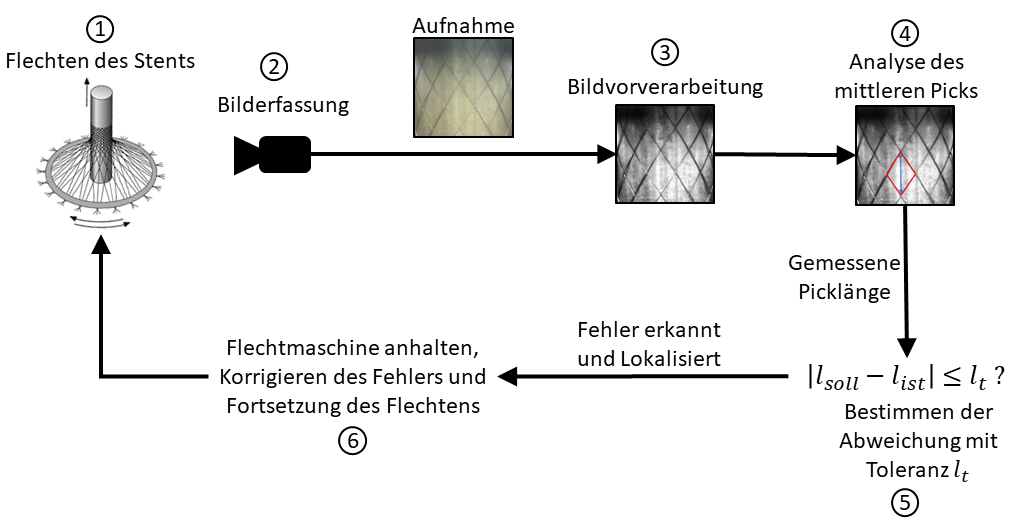
\includegraphics[width=15cm]{98_images/aufbau_projekt.png}
\caption{Aufbau des Gesamtsystems zur automatisierten Fehlererkennung und -korrektur von Stents basierend auf Kamerabildern}
\label{fig:aufbau_des_projekts}
\end{figure}


% Aufbau des Projekts
\section{Aufbau des Projekts}\label{sec:?}
Der grundlegende Aufbau des Systems für die automatische Fehlererkennung von Stents in der Produktion ist in Abbildung \ref{fig:aufbau_des_projekts} aufgezeigt. Die Stents werden bei einen vorgegebenen Flechtwinkel von einer Flechtmaschine hergestellt. Der Verlauf dieses Prozesses soll mit einer Kamera überwacht werden. Nach einer Vorverarbeitung der Bilder wird die Picklänge des mittleren Picks bestimmt und anhand der gewünschten Länge die Abweichung zwischen diesen zwei Werten berechnet. Mittels eines festgelegten Toleranzwertes wird entschieden, ob ein Fehler vorliegt oder nicht. Sollte ein Fehler im Geflecht vorhanden sein, wird die Flechtmaschine angehalten, der Defekt korrigiert und das Flechten im Anschluss fortgesetzt. Im Rahmen dieser Arbeit wurden drei dieser Schritte betrachtet: die Bildvorverarbeitung der Aufnahmen, deren Analyse, um die Länge des mittleren Picks zu bestimmen und die Bestimmung der Abweichung der Netzausgaben.


% Berechnung der Picklänge
\section{Berechnung der Picklänge}
Es gibt mehrere Ansätze, mit denen eine Pickanalyse durchgeführt werden kann. Schorle \cite{felix} untersuchte Methoden der Bildverarbeitung des klassischen maschinellen Lernens und faltende neuronale Netze, um den Mittelwert der Längen aller Picks in der Mitte des Bildes zu vermessen. Wie in Abbildung \ref{fig:abweichungen-vgl} dargestellt, kann trotz eines korrekten Mittelwertes ein Fehler in der Struktur des Stents vorliegen. Aus diesem Grund wird in dieser Arbeit nur der sich in der Mitte des Bildes befindende Pick analysiert. Aus den in \cite{felix} untersuchten Methoden wurden mit faltenden neuronalen Netzen die besten Ergebnisse erreicht. Deshalb werden sie im Rahmen dieser Arbeit für die Vermessung der Picklänge eingesetzt.

\begin{figure}[h!]
\centering
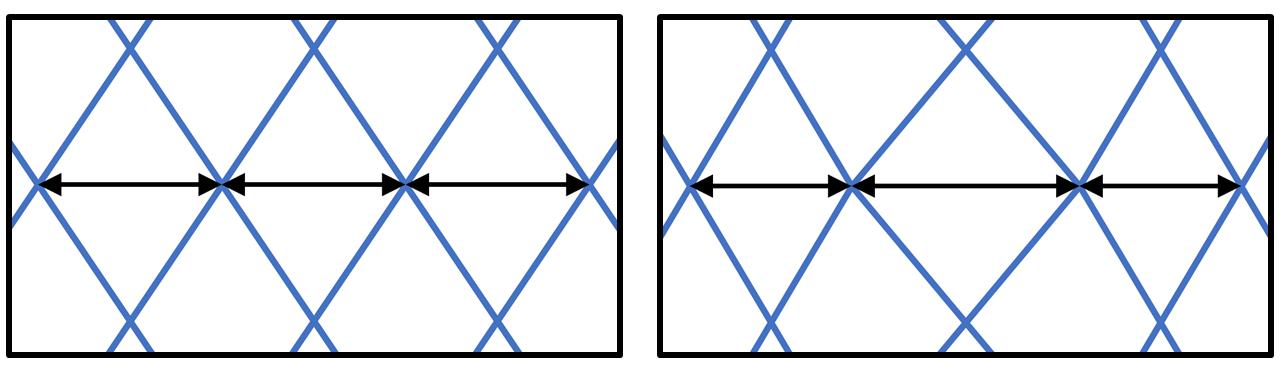
\includegraphics[width=13cm]{98_images/abweichungen_vgl.png}
\caption{Beispiel für zwei Zeilen von Picks mit gleicher durchschnittlicher Picklänge, fehlerfrei (links) und fehlerhaft (rechts)}
\label{fig:abweichungen-vgl}
\end{figure}


% Auswahl der CNNs
\section{Auswahl der faltenden neuronalen Netzen}\label{sec:auswahl-cnns}
Um möglichst vielfältige Netzwerkarchitekturen zu analysieren, wurden die in Kapitel \ref{sec:architekturen-grundlagen} beschriebenen Modelle implementiert und optimiert. Die Auswahl enthält sowohl aktuelle Architekturen wie EfficientNet, als auch Netze wie AlexNet, welche einen einfachen Aufbau haben. Zudem variieren die Einsatzgebiete der gewählten Architekturen.

\mypar Bei der Anwendung faltender neuronaler Netze mit Bildern gibt es drei große Anwendungsbereiche. Die meist verbreitete ist die Bildklassifizierung, welche Bilder in unterschiedliche Kategorien einstuft. Weiterhin wird die Objekterkennung angewendet, um beliebige Objekte innerhalb eines Bildes mit einem sogenannten Begrenzungskasten zu erkennen und einzurahmen. Im Vergleich dazu wird bei der semantischen Segmentierung jedem Pixel eine Kategorie zugeordnet. So kann das Bild in mehrere Bereiche oder Cluster aufgeteilt werden. Einige Beispiele zu diesen Bereichen sind in Abbildung \ref{fig:cnn-anwendungen} aufgezeigt. In der Netzauswahl befinden sich Netze, die auch für weitere Anwendungen eingesetzt werden. Dazu zählen die Maschinenübersetzung, bei der Texte aus einer Sprache in eine andere umgewandelt werden können und die Superauflösung, welche sich mit der Verbessung der Auflösung von Bildern auseinandersetzt.

\begin{figure}[h!]
\centering
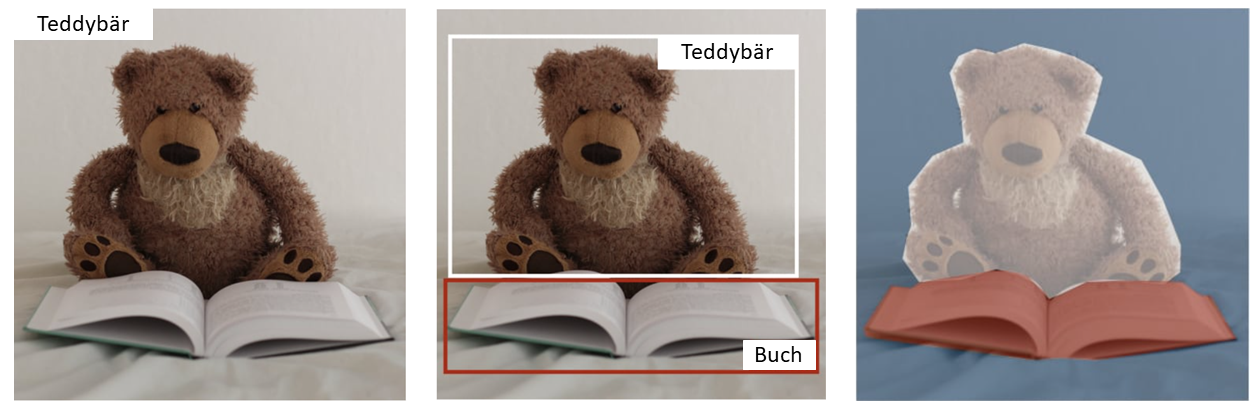
\includegraphics[width=15cm]{98_images/cnn_anwendungen.png}
\caption{Beispiele für die drei größten Anwendungsbereiche von CNNs: Klassifizierung (links), Objekterkennung (Mitte), Segmentierung (rechts). Ursprüngliche Bilder aus \cite{amidi2018convolutional}.}
\label{fig:cnn-anwendungen}
\end{figure}


% Erfassung der Trainingsdaten
\section{Erfassung der Trainingsdaten}\label{sec:erfassung-trainingsdaten}
Das Trainieren von neuronalen Netzen erfordert einen Datensatz. Hierfür wurden Bilder von Stents inklusive der zugehörigen Picklängen als Labels verwendet. Die vom Projekt Stents4Tomorrow \cite{flechtmaschine} zur Verfügung gestellten Bilder zeigen mehrere Segmente von Stents mit unterschiedlichen Flechtwinkeln. Diese Bilder der Größe $3088 \times 2064$ enthalten Informationen, wie der Hintergrund, welche für die Vermessung der Picklänge irrelevant sind. Zudem wird ein sehr langer Abschnitt des Stents gezeigt, wodurch nicht immer ein Pick in der Mitte des Bildes zu sehen ist. Aus diesem Grund wurden zur Verfügung gestellte vorgeschnittene Bilder der Größe $450 \times 450$ verwendet, um die neuronalen Netze zu trainieren. Ein Beispiel für eines der ursprünglichen Bilder und ein vorgeschnittenes Bild ist in Abbildung \ref{fig:bild_normal_vorgeschnitten} zu sehen. Als Label für die Bilder wird die Länge des mittleren Picks im Bild in Pixel angegeben.

\begin{figure}[ht!]
\centering
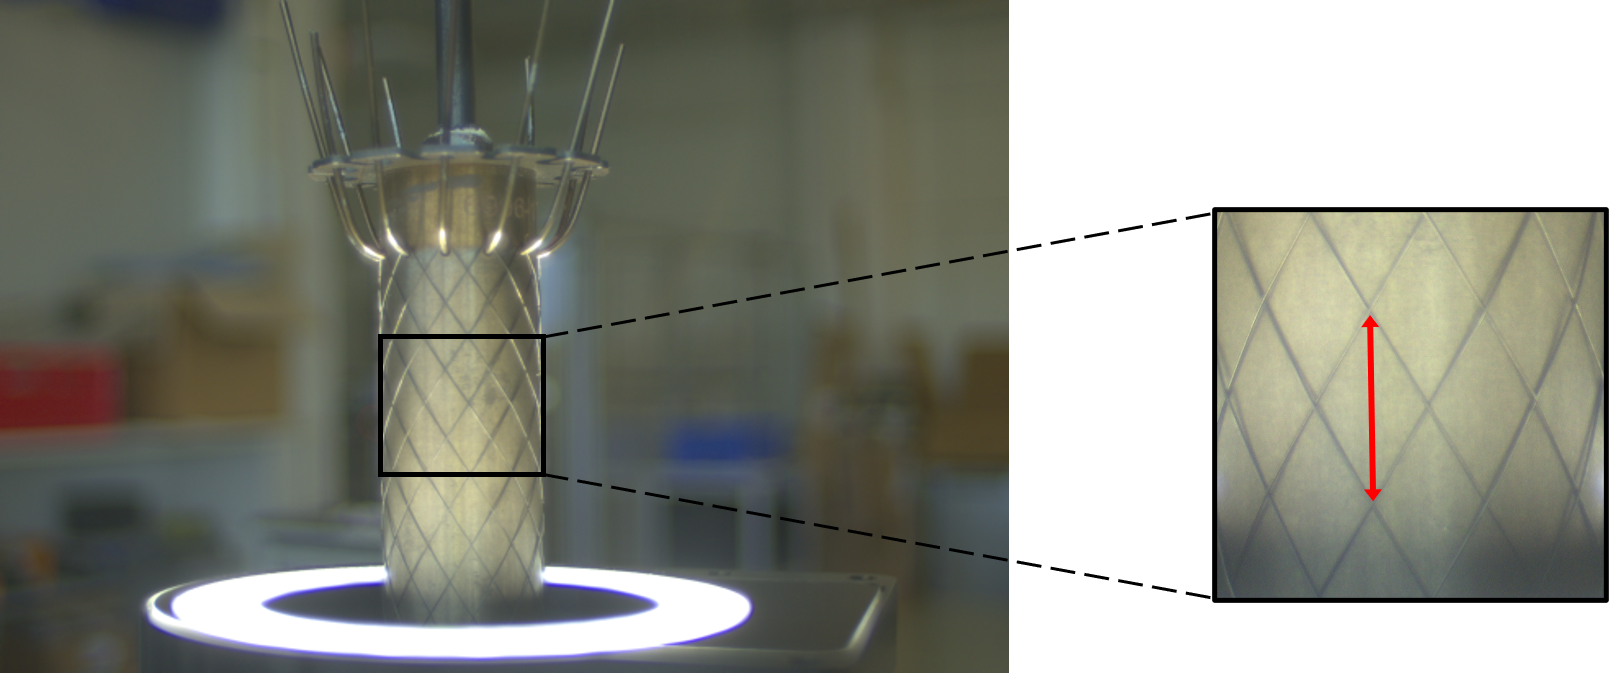
\includegraphics[width=12cm]{98_images/stent_normal_cropped.png}
\caption{Ursprüngliches Bild der Größe $3088 \times 2064$ (links) und vorgeschnittene Variante (rechts). Die Länge des sich in der Mitte des in der Bildmitte befindlichen Picks ist rot eingezeichnet.}
\label{fig:bild_normal_vorgeschnitten}
\end{figure}








